\chapter{Eredmények}
\pagestyle{headings}

\def\s{0.5}
Munkám során próbáltam lépésről lépésre haladni, valamint az egyes lépések eredményeiről beszámolni. Fontosnak tartottam a korábban, mások által végzett munka főbb állomásainak reprodukálását, és azok begyakorlását. Csak akkor tértem át a következő, bonyolultabb vizsgálatra, mikor az azt megelőző, alapként szolgáló eredményeket sikeresen reprodukáltam. Az oszcilláló reakció vizsgálata előtt meggyőződtem róla, hogy a használt potenciometriás mérőcella elég gyorsan tudja-e követni a reakcióban fellépő potenciálváltozást. Ehhez egy \emph{,,flip--flop''} áramkört használtam, mely nagyon gyors potenciálugrás produkálására képes. A \ref{fig:square}. ábrán látható, hogy a mérőműszer követni tudja a gyors potenciál-változásokat. A használt mérőrendszerrel tehát vizsgálható a Belouszov-Zsabotyinszkij reakció.

\begin{figure}
\centering
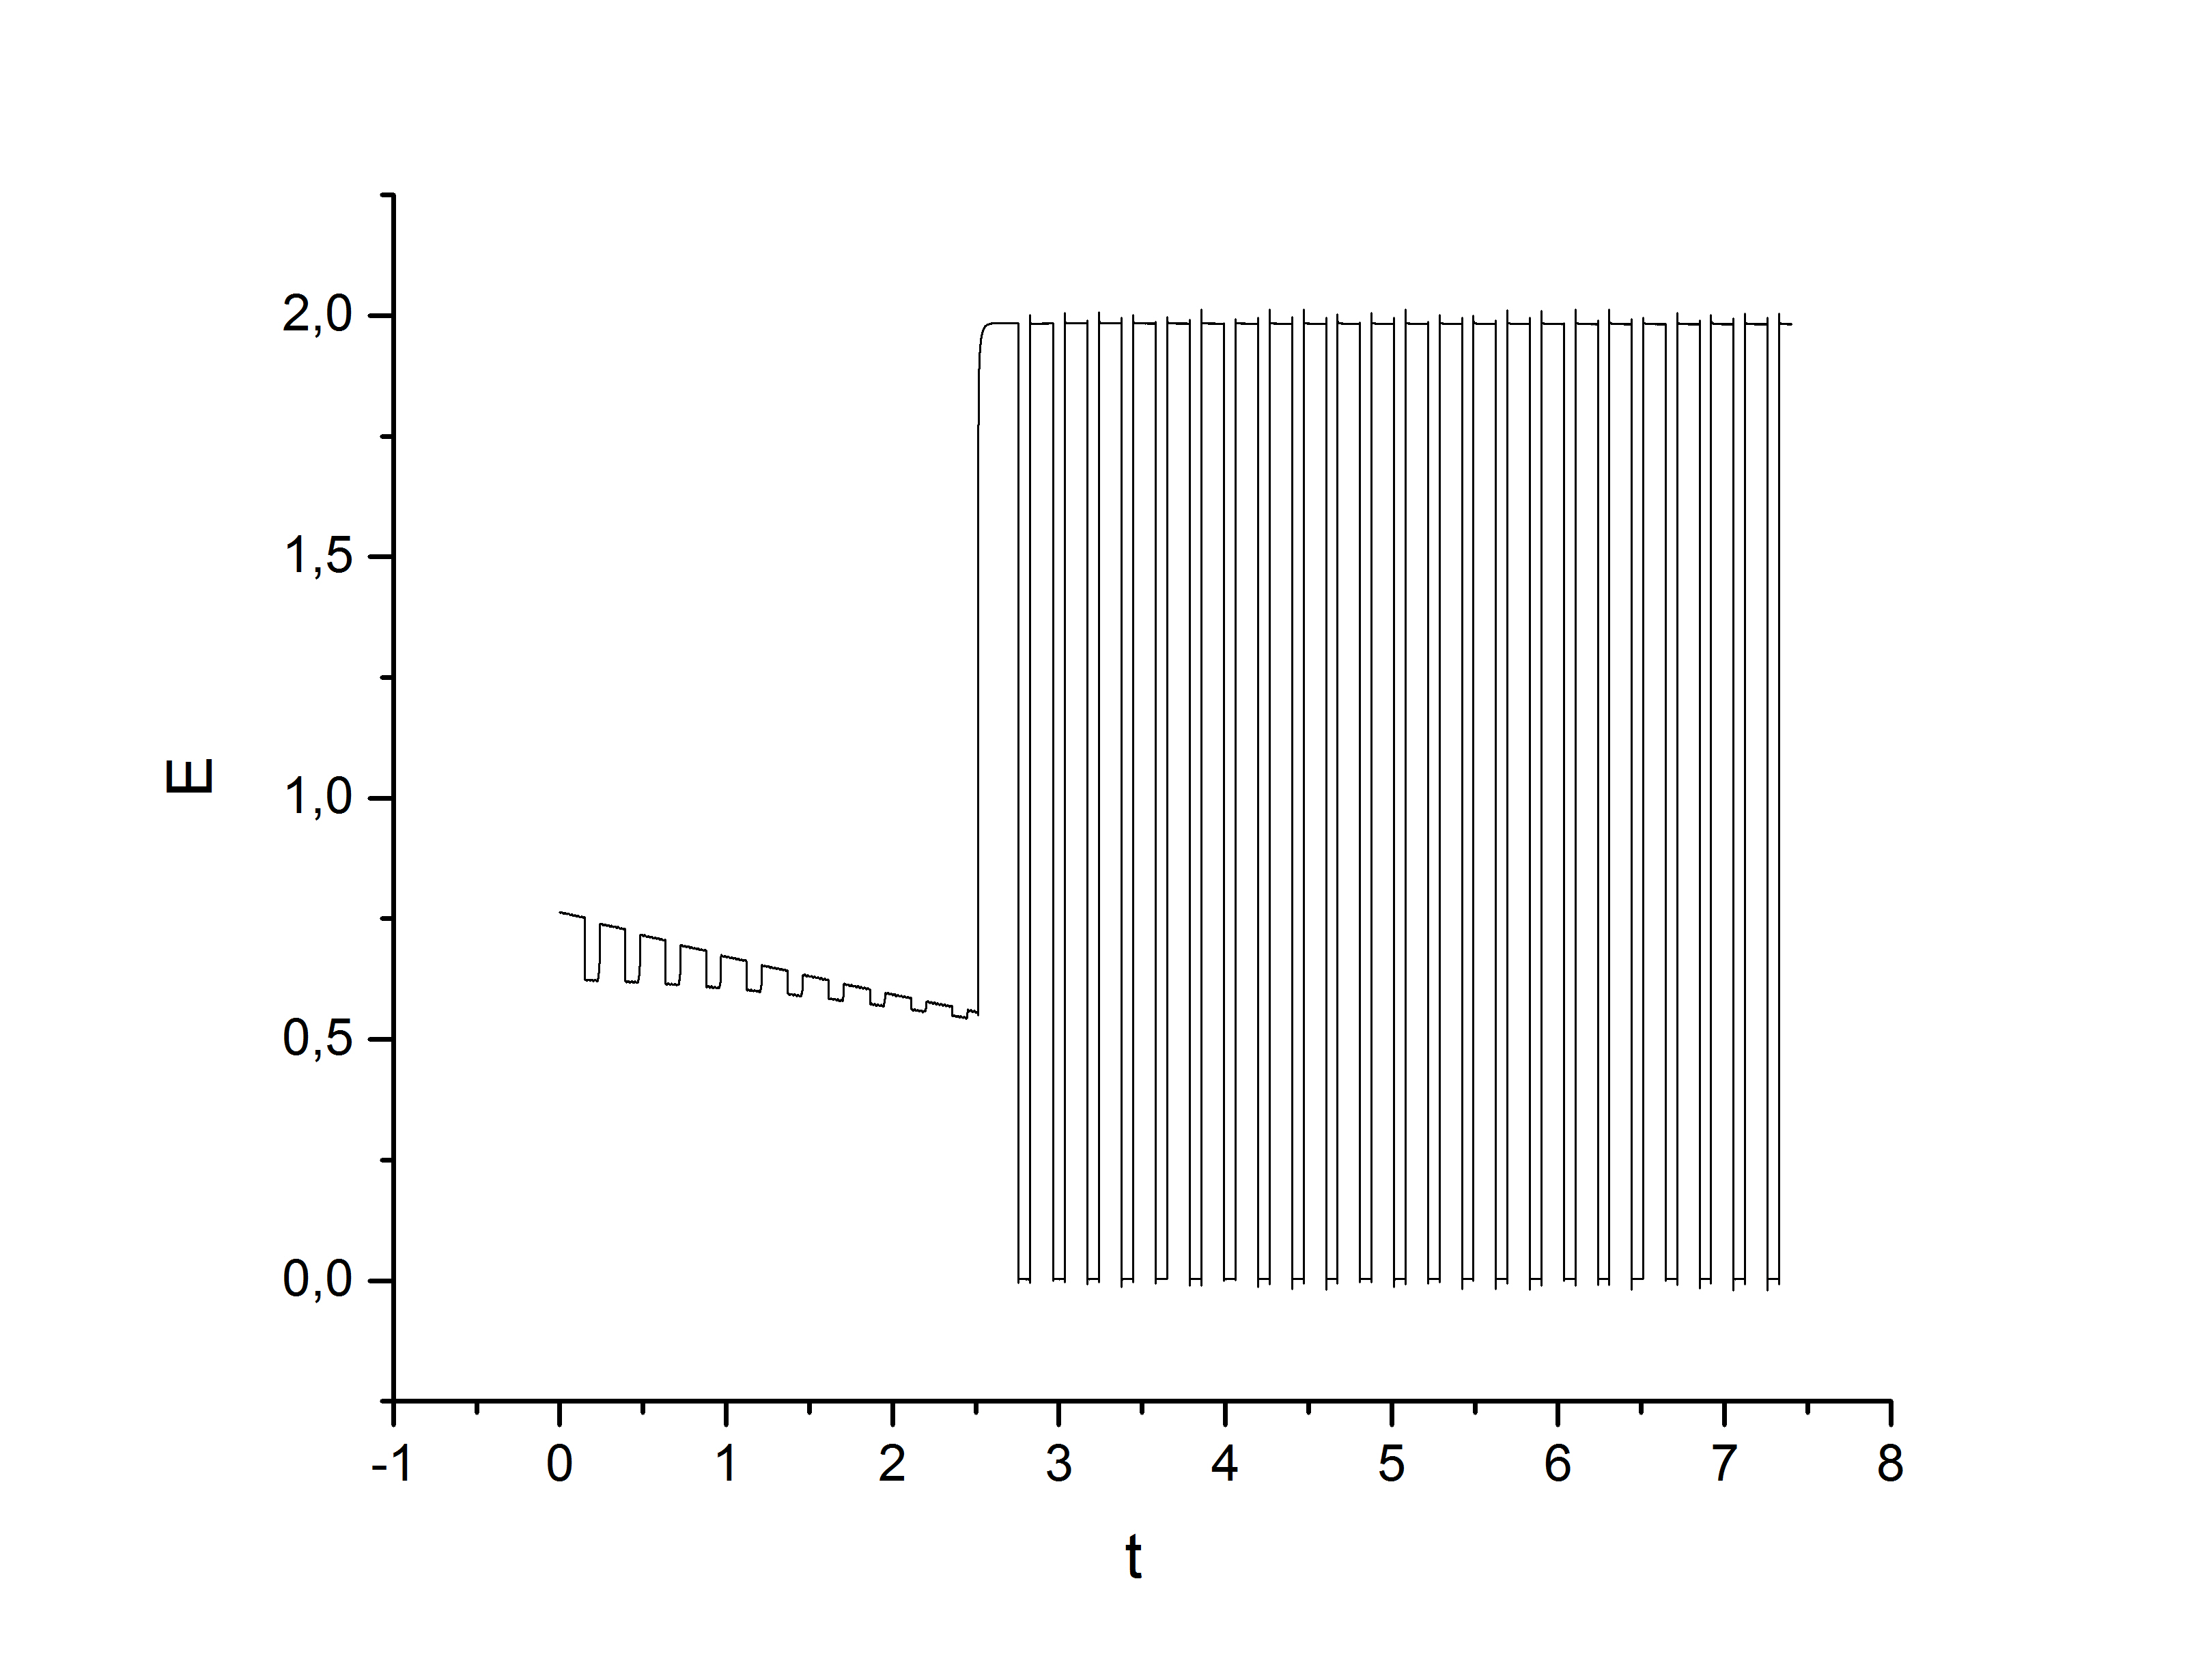
\includegraphics[width=0.8\textwidth]{img/square.jpg}
\caption{A "flip-flop" 2 V-os, 200 ms-os négyszöghullámra mért potenciálváltozások.}
\label{fig:square}
\end{figure}

\section{Platina elektród}
A Belouszov-Zsabotyinszkij reakció tanulmányozását a gyárilag előállított makroméretű elektródokkal kezdtem a mérés begyakorolása valamint Kőrös Endre eredményeinek \cite{noyes1972oscillations} reprodukálása végett. Miután begyakoroltam a módszert, a saját készítésű elektróddal kezdtem el vizsgálni a már említett reakciót. A vizsgálatok során először kevertetve tanulmányoztam az oldatot, a kevertetést mágneses keverő segítségével valósítottam meg. A kevertetett reakció többszöri vizsgálata után kevertetést nem használva vizsgáltam a rendszert.
\begin{figure}[h]
\centering
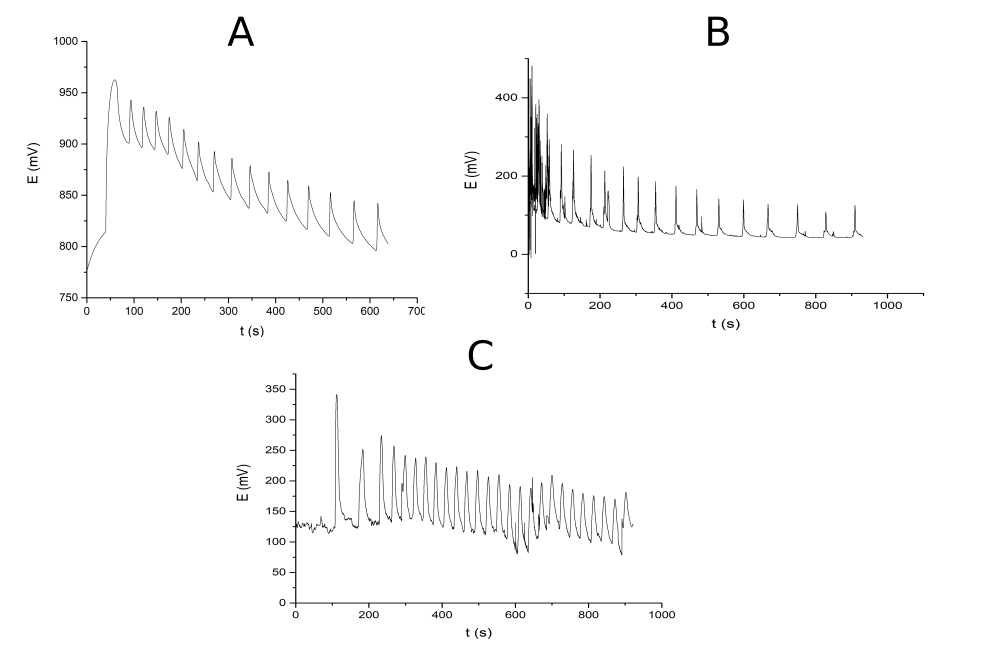
\includegraphics[width=1\textwidth]{img/platina_meres.png}
\caption{A BZ-reakció tanulmányozása platina elektródokkal. (A) a kevert reakció vizsgálata makroméretű platina elektróddal, (B) kevert reakció platina mikroelektróddal, (C) keveretlen reakció vizsgálata platina mikroelektróddal. A potenciált az Ag/AgCl referencia elektródhoz viszonyítva mértem.}
\label{fig:platina_meres}
\end{figure}
A \ref{fig:platina_meres}.A ábrán látható a kevert rendszer vizsgálata makroméretű platina elektróddal. A vizsgálatból megfigyelhető, hogy a kevertett reakció esetében a periódusidő az idő függvényében közel lineárisan csökken. A \ref{fig:platina_meres}.B képen az adott kevert reakció tanulmányozása mikroméretű platina elektróddal. A \ref{fig:platina_meres}.C ábrán az előző alkalommal vizsgált rendszer keverés nélkül. A vizsgálatok során mértem a platina elektródokon kialakult potenciál a referencia elektródhoz (Ag/AgCl) képest. A \emph{"Célkitűzés"} című fejezet 1. pontjában megemlített Field, Noyes és Kőrös eredményeit \cite{noyes1972oscillations} sikeresen reprodukáltam.  

\section{Szénszál elektród}
A platina elektródok sikeres alkalmazása után szénszál elektródokkal folytattam a reakció vizsgálatát. Ezen mérések során a potenciálban hasonló változásokat véltem felfedezni, amit a \ref{fig:pontszerumeres}. ábrán a színes optikai kép előtt látható fekete vonallal jelzett elektrokémiai jel mutat. Mivel a redoxpotenciált a platina elektródhoz hasonlóan tudtam követni a szénszál elektródokkal, alkalmasnak bizonyultak a reakció tanulmányozásához. Későbbi munkám során már csak szénszál elektródokkal tanulmányoztam a rendszert, a platina elektród mérétének további csökkentése miatt (kisebb platina szál nem állt rendelkezésre).
\subsection{Mérés egy pontban}
A keveretlen reakció elektrokémiai tanulmányozását optikai módszer felhasználásával tovább bővítettem. Az előző pontban végzett vizsgálatok alapján és a későbbiekben előkerülő miniatürizálás érdekében szén mikroelektródokkal folyattam a vizsgálatokat. Az elektrokémiai jelet optikai képpel kombináltam,ennek eredményét  mutatom be ezen a pontban. Az optikai képet az \emph{"Optikai tér-idő kép szerkeztése"} című fejezetben leírt módszer alapján készítettem.
\begin{figure}[h]
\centering
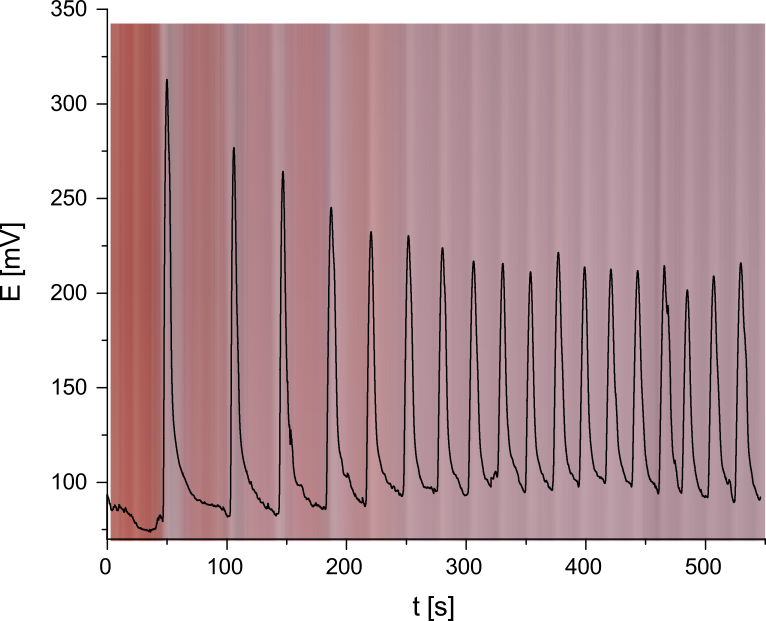
\includegraphics[width=0.8\textwidth]{img/pontszerumeres.png}
\caption{Pontszerű elektrokémiai és optikai mérés. A háttérben látható optikai kép, ahol a kék szín a ferroin indikátor oxidált-, míg a piros szín a redult formáját mutatja. Előtte fekete vonallal jelölve látható a mért elektrokémiai paraméter, a redoxpotenciál. Az optikai és az elektrokémiai méréseken megfigyelhető, hogy az oxidált hullámoknak megfelelő csúcsok egybeesnek.}
\label{fig:pontszerumeres}
\end{figure}

A \ref{fig:pontszerumeres}. ábrán látható az optikai képhez az elektródpotenciált rendelve. A képen a kék szín az oxidált, a piros szín a redukált formához rendelhető. Az ábrán látszik, hogy a két mérésen megfigyelhető oxidáló hullámok helye rendkívül jól egyezik. A reakció jól vizsgálható tehát a hazsnált mikroelektróddal. A következő logikus lépés a mikroelektród mozgatása volt, amire a következő pontban térek ki.

\subsection{Elektrokémiai pásztázás az oldatfázis felületén}
Az elektrokémiai és optikai módszert tovább gondolva kezdtem meg a PEKM alkalmazását, amellyel elektrokémiai és optikai tér idő képet kaptam. Ezeknek a képeknek a kombinálását mutatom be ebben a pontban. A két módszer kombinálásának előnye, hogy térbeli kémiai információt kapunk az adott felületről.
\begin{figure}[h!]
\centering
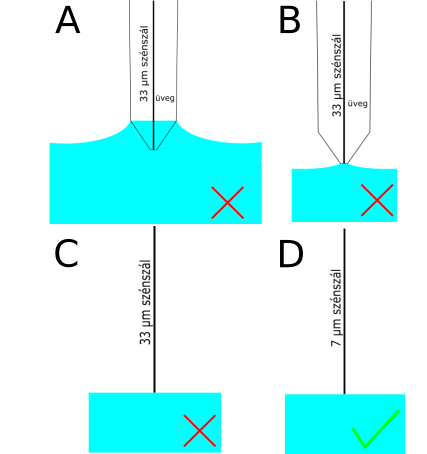
\includegraphics[width=0.8\textwidth]{img/oldat.png}
\caption{A pásztázás során a mikroelektródok helyzete az oldathoz képest. Üvegszigeteléssel ellátott szénszál mikroelektród az oldatban (A) és az oldat felületén (B). 33 $\upmu$m (C) és 7 $\upmu$m (D) szénszál az oldat felületén. Csak a (D) esetben nem tapasztaltam konvektív zavarást a pásztázás közben.}
\label{fig:oldat}
\end{figure}
A PEKM használatát a 33 $\upmu$m átmérőjű szén-mikroelektróddal próbáltam eleinte megvalósítani, de az elektród az oldatba merülve konvektív zavarást okozott a reakcióban(\ref{fig:oldat}.A ábra). Mivel a vizsgált reakció eleve kvázi--kétdimenziós és a vertikális grádiensek elhanyagolhatóak, a zavarás elkerülésének érdekében az elektródot csak egy pontban érintettem az oldathoz (\ref{fig:oldat}.B ábra). Sajnos még mindig konvektív zavarást véltem felfedezni a pásztázás során. Mivel az elektród egy pontban érintkezett a vizsgálandó oldattal, az elektród üveg szigetelését elhagyhattam (\ref{fig:oldat}.C ábra), azonban így sem jártam sikerrel. Az előzőekben leírt kíserletezések sikertelensége arra engedett következtetni, hogy ez a mérés a 33 $\upmu$m-es elektróddal nem fog sikerülni. Ezért magát a szénszál elektródot kellett finomítani, mivel nagy konvektív hatása van a pásztázás során (szemmel látható kavarodást okoz a reakcióelegyben), ami a "nagy" átmérőből fakad. Ennek kiküszöbölésére egy 7 $\upmu$m átmérőjű szén-mikroelektródot alkalmaztam (\ref{fig:oldat}.D ábra). Ezzel a szénszállal sikerült a zavarás mentes pásztázás, nem lépett fel szemmel látható konvekció. A fellépő zavarást a rendszer diffúzió által ellensúlyozni tudta. A kémiai hullámok a reakciótér faláig zavaratlan formában haladtak tovább. Ez a  vizsgálat látható a \ref{fig:secmkep}. ábrán.
\begin{figure}[h]
\centering
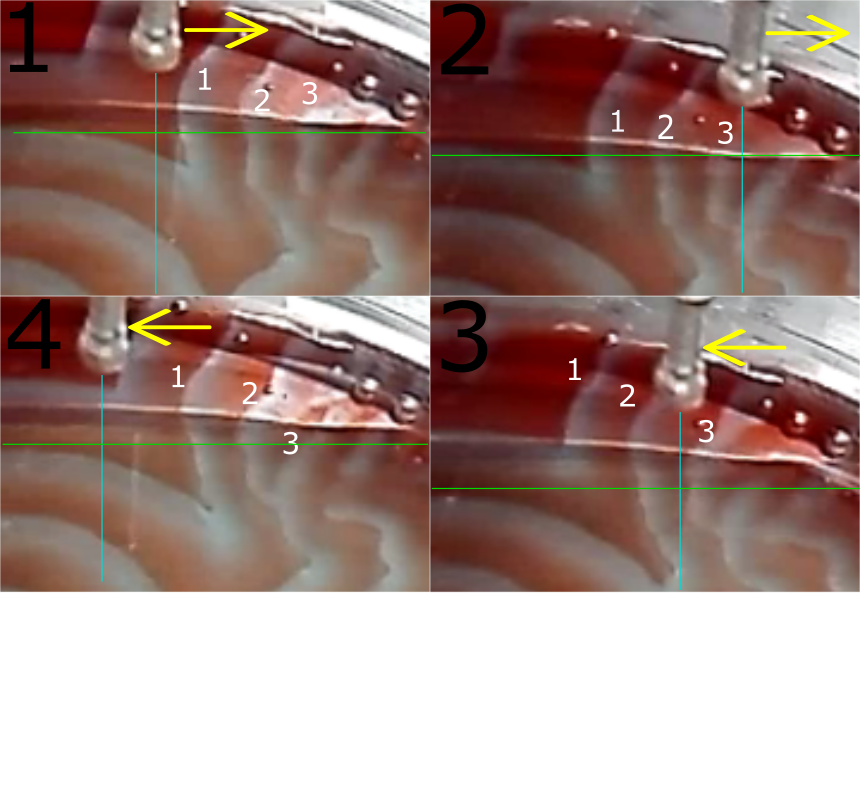
\includegraphics[width=0.8\textwidth]{img/secmkep.png}
\caption{Az ábrán a fekete nagy számok a mérés időbeli változását mutatják 1-4 sorrendben. A kis fehér számok a hullámok sorszámát mutatja. A vízszintes zöld vonal a pásztázás vonalát mutatja, a függőleges kék vonal az elektród test helyét mutatja. A zöld és a kék vonal keresztezésénel található az elektródtest vége, ami 1 $\upmu$m-re merült a vizsgálandó BZ-reakcióelegybe. Szemmel látható, hogy az elektródtest nem okozott konvektív zavarást a pásztázás során.}
\label{fig:secmkep}
\end{figure}

\begin{figure}
%% trim = top left bottom right
\centering
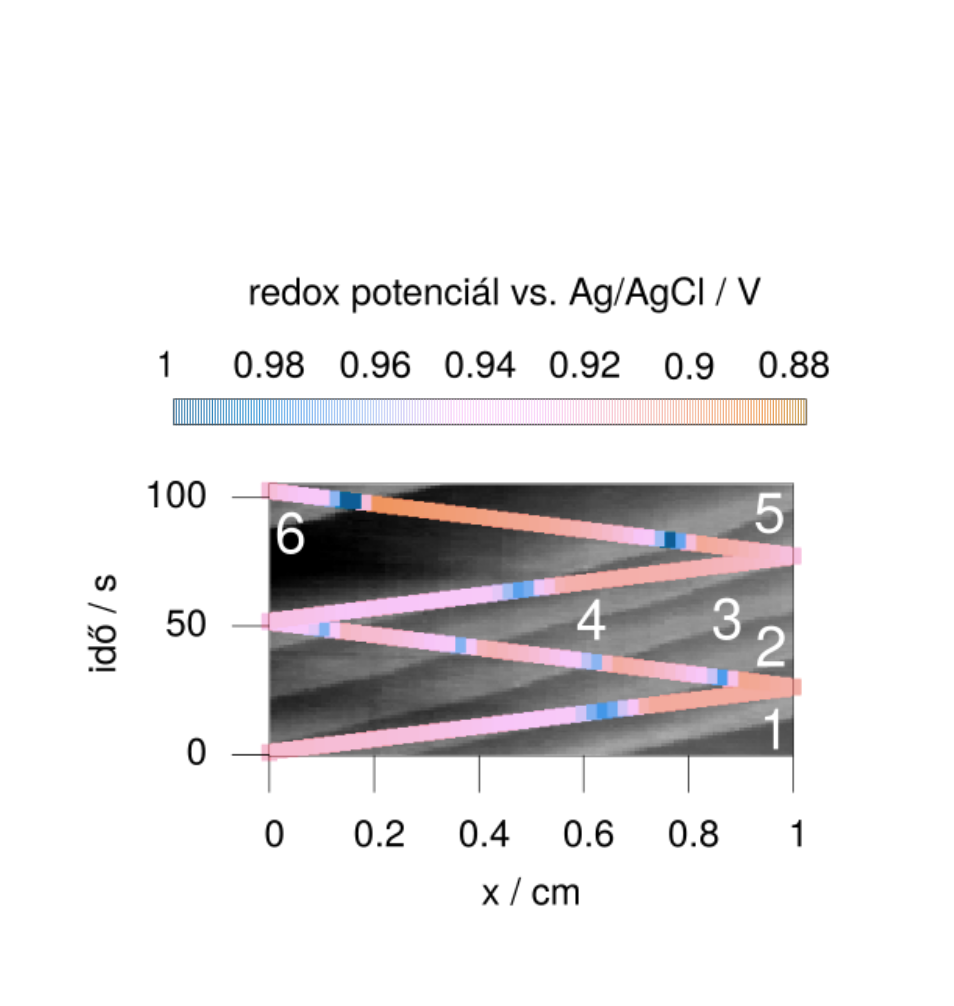
\includegraphics[width=0.8\textwidth]{img/spacetime2.eps}
\caption{Az ábra egy elektrokémiai tér-idő képet ábrazol egy optikai tér-idő képpel a háttérben. Az optikai képet az \emph{"Optikai tér-idő kép szerkeztése"} című fejezetben leírt módszer alapján készítettem. Az háttérben látható világosabb sávok a BZ-reakció oxidációs hullámjai. A két ciklusos pásztázás során kapott elektrokémiai paraméter (redoxpotenciál) tökéletesen egybevág az optikai képpel, ezt az ábrán a \emph{cikk-cakk} vonalakon elhelyezkedő kék szín ($\approx$ 1 V) mutatja, ami a redoxpotenciál maximum értékei az oxidáló hullám esetében.}
\label{fig:spatiotemporal}
\end{figure}
Munkám fő eredményét a \ref{fig:spatiotemporal}. ábra mutatja. Látszik, hogy jó egyezést kaptam az optikai és az elektrokémiai mérés között. Tudtommal ilyen eredmény eddig nem született. A PEKM előnye az optikai módszerrel szemben, hogy olyan köztitermékek is vizsgálhatók, melyek nem színesek. Olyan esetekben is hasznos lehet a módszer, mikor a köztitermékek elnyelési spektrumai egybeesnek. Elektrokémiai módszerekkel nagyfokú szelektivitás érhető el. Jól térképezhető lenne például a bromid-ion aktivitás.

A kapott adatok egy alkalmazását szeretném bemutatni példaként. Az ábráról, valamint a készülék által rögzített koordináta, idő, potenciál adatokból meghatározhatjuk például azon hullámok sebességét, melyekkel a pásztázás során többször is találkozott a mérőcsúcs. Ezeket az adatokat \ref{hullam}. táblázatban foglaltam össze, és számítottam ki a hullámok terjedési sebességét.

\begin{table}[h] 
\centering
\caption{\ref{fig:spatiotemporal}. ábráról leolvasható a mérés során kapott elektrokémiai jelek maximumai és a hozzájuk tartozó térkoordináta és idő adatok. Ezek segítségével a megjelölt kémiai hullámokról különböző statisztikai adatok számíthatóak.}
\label{hullam}
\begin{tabular}{|c|c|c|c|c|}
\hline
\textbf{Hullám sorszáma} & \textbf{t (s)} & \textbf{E (mV)} & \textbf{x (mm)} & \textbf{v ($\upmu$m/s)}        \\ \hline
\multirow{2}{*}{2}       & 17             & 978             & 6,4             & \multirow{2}{*}{169,23} \\ \cline{2-4}
                         & 30             & 977             & 8,6             &                         \\ \hline
\multirow{3}{*}{5}       & 49             & 968             & 1               & \multirow{3}{*}{191,3}  \\ \cline{2-4}
                         & 64             & 975             & 4,8             &                         \\ \cline{2-4}
                         & 83,5           & 1027            & 7,6             &                         \\ \hline
\end{tabular}
\end{table}
